\section{Introducción}

La industria de vehículos eléctricos se encuentra en crecimiento debido a la
necesidad de utilizar energías limpias y renovables para reducir los efectos 
causados por el cambio climático y la contaminación ambiental. Dentro de esta 
industria, la carga rápida es una de las principales características a ser 
mejorada. Para dar una idea del desafío con el cual nos encontramos, el tiempo 
de recarga de la batería de los autos eléctricos de Nivel 2 se encuentra entre 
las 4 y las 10 horas \cite{evcs}. Este número es dos ordenes de magnitud 
mayor que el tiempo que toma recargar un auto a combustión interna.

Existen distintos criterios para definir que una carga sea rápida. Un criterio 
pensado para la aplicación de vehículos eléctricos, busca una autonomía de 30 km 
por minuto de carga \cite{dufek2022}. Otro criterio, definido por el USABC (de sus
siglas en inglés, \textit{United States Advanced Battery Consortium}), tiene como
objetivo obtener el 80\% del Estado de la Carga (SOC, \textit{State-of-Charge})
en 15 minutos \cite{USABC}. Este último es el criterio elegido para esta tesis.
Para cumplir con el mismo, es necesario entender la física de los materiales de
intercalación y como estos se comportan durante el cargado, ya que esto podría 
permitir una optimización en el diseño de los electrodos.

La carga rápida es un problema multi-escala \cite{franco2013, franco2019} y, por 
lo tanto, las mejoras en la velocidad de carga de las celdas electroquímicas 
requieren una comprensión desde el nivel atómico hasta el ingenieril. Dentro 
de lo que es la escala micrométrica, los procesos que determinan la velocidad de 
carga al nivel de una sola partícula de los materiales de electrodos son la 
difusión de iones de litio dentro de electrodos y la transferencia de carga en 
las interfases electrodo/electrolito, por lo cual es necesario favorecer ambos
procesos \cite{liu2019, tomaszewska2019, weiss2021}. También se ha mostrado
que el tamaño y la geometría de las partículas juegan un rol importante en el 
desempeño electroquímico \cite{gavilan2020, gavilan2022}. Así, incluso descartando
otros factores que podrían influir en la carga de la batería (como cambios de 
volumen durante la intercalación de iones de litio, termodinámicas particulares
de los sistemas, formación de interfase electrolito/sólido, etc), es complicado
realizar un análisis detallado del desafío general.

La electroquímica de electrodos de una sola partícula \cite{ventosa2021, 
heubner2020, takahashi2020, wahab2020, xu2020, tao2019, fukui2011} permite 
estudiar la respuesta \say{pura} de los materiales activos, i.e., sin el efecto 
de otros aditivos presentes en los electrodos compuestos. Esta información 
detallada es valiosa ya que nos da a conocer los factores limitantes para su 
carga rápida y su respuesta frente a la misma. Enmarcado en este contexto, un 
modelo de una sola partícula recientemente propuesto \cite{gavilan2023} fue 
utilizado para construir diagramas galvanostáticos de la capacidad máxima 
alcanzada por una sola partícula en función de dos parámetros adimensionales: uno
cinético,
\begin{equation}\label{eq:xi}
    \Xi = k^0 \sqrt{\frac{t_h}{C_r D}},
\end{equation}
y el otro de difusión finita,
\begin{equation}\label{eq:ele}
    \ell = d \frac{V}{A} \frac{C_r}{D t_h},
\end{equation}
donde $k^0$ es la constante cinética, $D$ el coeficiente de difusión, $V/A$ es la 
proporción volumen/superficie, $d$ es el tamaño característico de la partícula, 
$C_r$ denota la \textit{C-rate} y $t_h$ el tiempo de una hora (en unidades 
correspondientes). En la Figura \ref{fig:diagnostico}a se muestra en 2D la 
capacidad alcanzada en función de los dos parámetros adimensionales, estos valores 
se corresponden con los cortes de los perfiles galvanostáticos presentes en las
Figuras \ref{fig:diagnostico}b y c (ejemplos para algunos valores en particular 
de $\Xi$ y $\ell$) a 150 mV debajo del potencial de equilibrio.

\begin{figure}[h!]
    \centering
    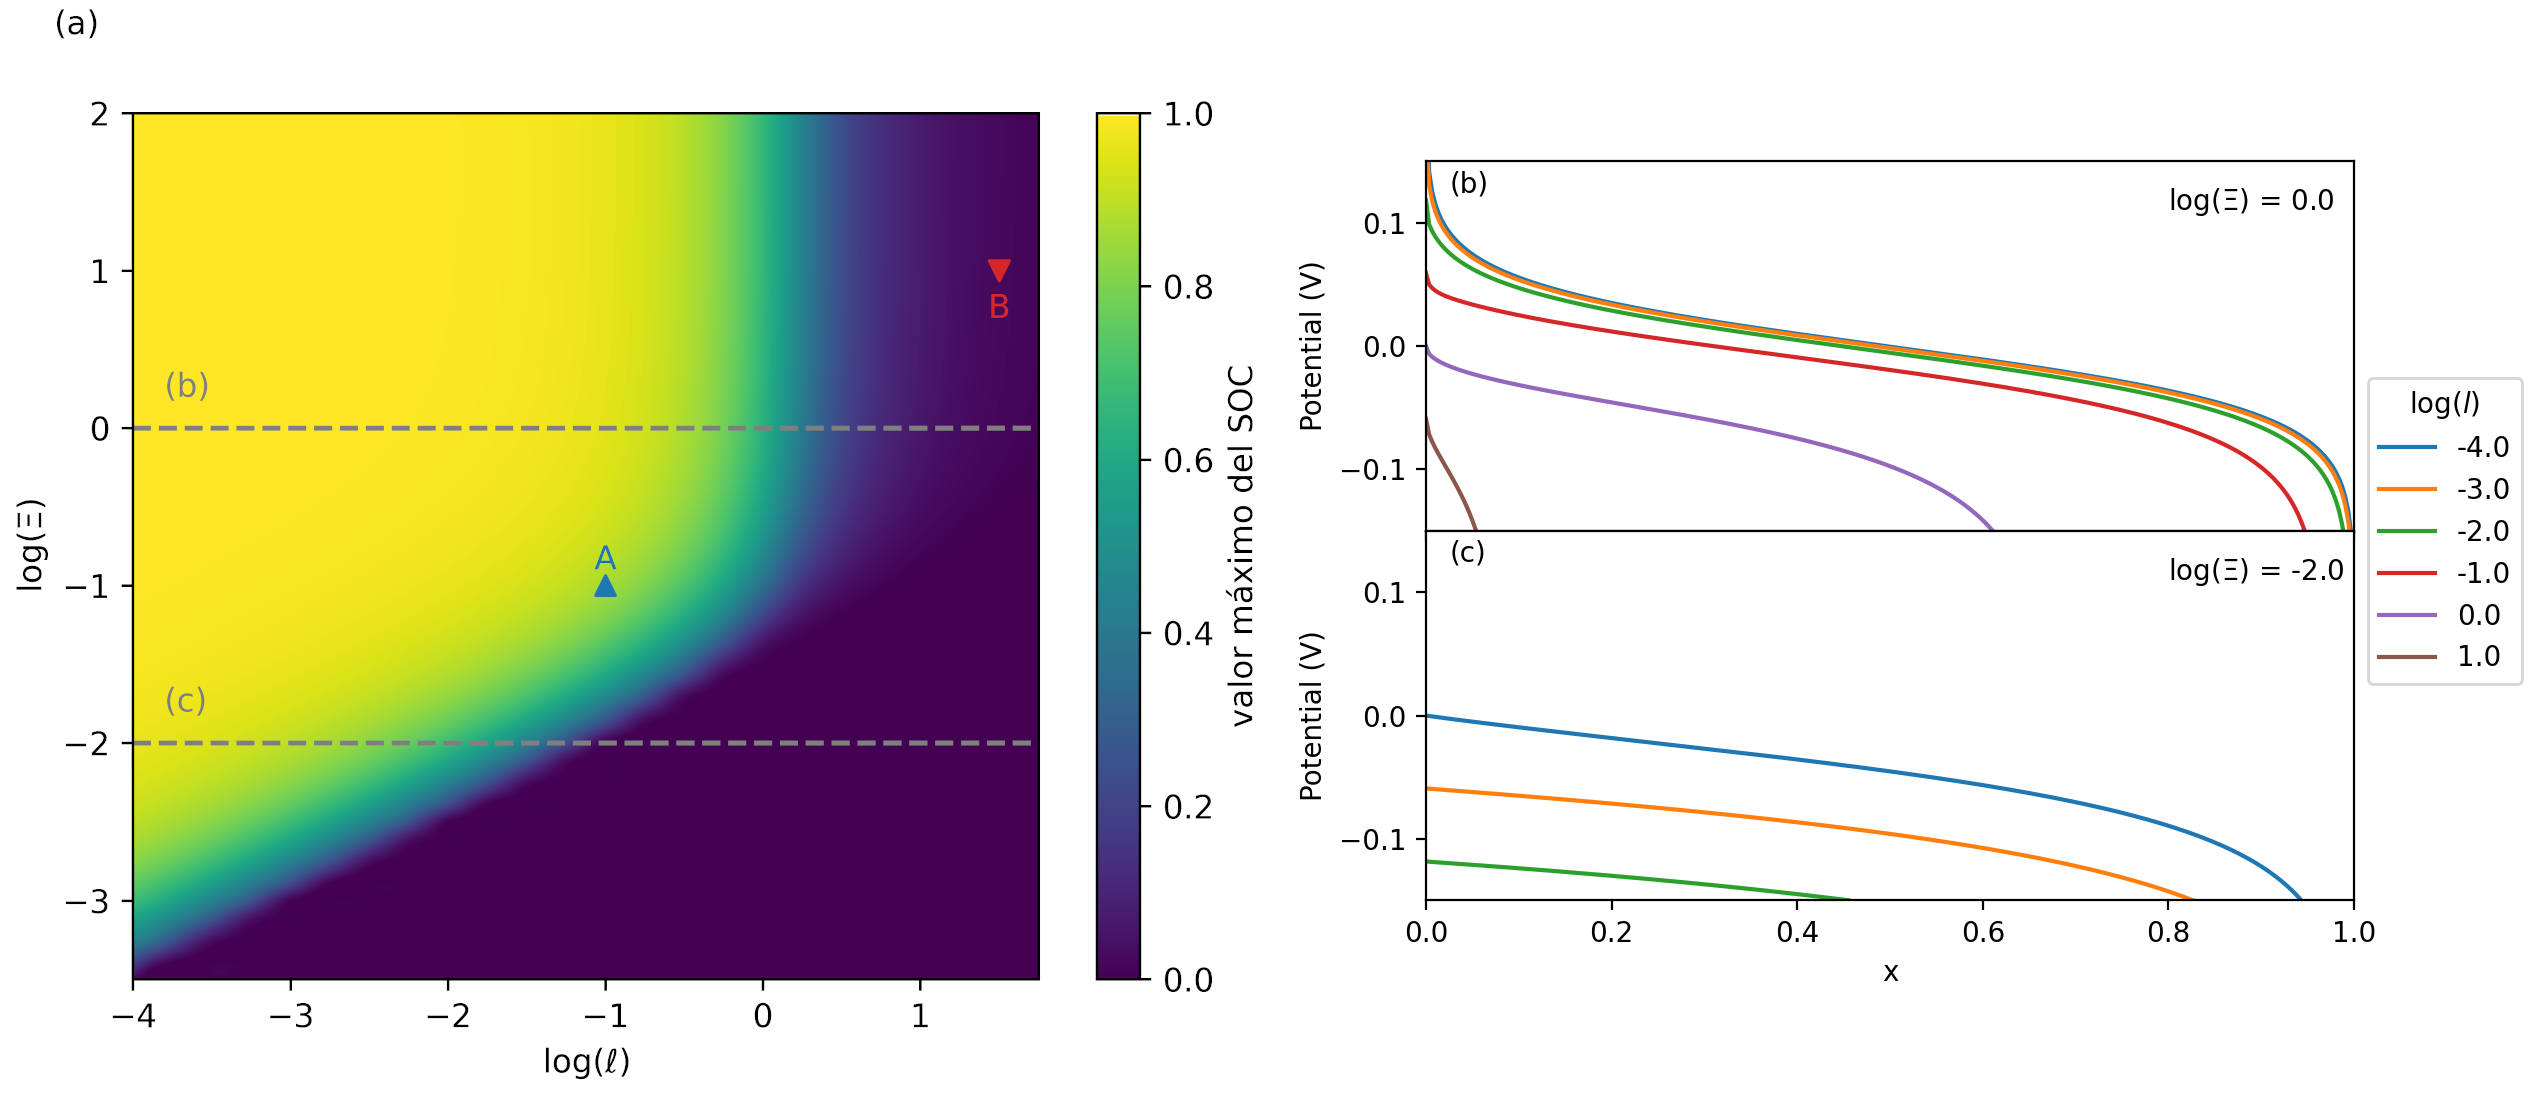
\includegraphics[width=\textwidth]{FastCharging/un/introduccion/diagnosis-merged.png}
    \caption{(a) Diagrama de nivel para una geometría esférica con un voltaje de 
    corte de 150 mV y condiciones de contorno detalladas en la sección 
    \ref{s:metodologia}. Los datos de los puntos A y B se encuentran en la 
    Tabla \ref{t:ab}. (b) y (c) muestran perfiles voltaje/capacidad para 
    diferentes valores de $\Xi$ y $\ell$, ver líneas grises punteadas en 
    Figura \ref{fig:diagnostico}a.}
    \label{fig:diagnostico}
\end{figure}


Los parámetros $\Xi$ y $\ell$ introducidos en las ecuaciones \ref{eq:xi} y 
\ref{eq:ele}, respectivamente, son relaciones de escaleo útiles para hacer una
primera predicción cualitativa de la capacidad que un material alcanzaría a una
dada C-rate. Esto es relevante ya que permite realizar la tarea no-trivial de
clasificar distintos materiales, cada uno caracterizado por los descriptores $D$,
$k^0$ y $d$.

Las relaciones de escaleo suelen dar una respuesta simple, aunque aproximada, a 
problemas complejos, esta cualidad ha hecho que tengan una gran popularidad 
en la física y en la química. Quizás uno de los casos más conocidos sea el de los
gases ideales
\begin{equation}
    \frac{p V}{n T} = R,
\end{equation}
que no es más que escalear el producto de la presión y el volumen, $p V$, por la
temperatura absoluta, $T$, y el número de moles, $n$, para obtener una constante
universal. Aunque de forma aproximada, esta ecuación proporciona una guía 
importante para resolver muchos problemas prácticos y es utilizada como referencia
para entender el comportamiento de fluidos más complejos que los gases ideales.

De manera similar a la de los gases ideales, el valor máximo del SOC alcanzado a 
un dado potencial de corte y a una dada C-rate, SOC$_{\max}$, puede 
pensarse como una función universal de los parámetros de escaleo $\Xi$ y $\ell$,
\begin{equation}\label{eq:socmax}
    \text{SOC}_{\max} = f(\Xi, \ell) = f(d, D, k^0, C_r).
\end{equation}
Esta cantidad puede ser obtenida en un mapeo ($\Xi$, $\ell$) de simulaciones 
galvanostáticas, como se la presenta en la Figura \ref{fig:diagnostico}a.

Un trabajo reciente ha propuesto una figura de mérito que permite establecer 
una jerarquía entre distintos materiales de carga rápida \cite{xia2022}. Desde
este punto de vista, la ecuación \ref{eq:socmax} evaluada en el punto ($\Xi$, 
$\ell$) se introduce como una figura de mérito. Supongamos que tenemos dos 
materiales, A y B, con las propiedades dadas en la Tabla \ref{t:ab} y se quiere
determinar si alguno de ellos es un buen candidato para una carga en 15 minutos.
Entonces, con los datos de las columnas 2--4 de la Tabla \ref{t:ab} podemos 
calcular los valores de $\Xi$ y $\ell$, utilizando las ecuaciones \ref{eq:xi} y
\ref{eq:ele}, presentados en la quinta y la sexta columna de la Tabla \ref{t:ab}.
Los puntos correspondientes a estos materiales se presentan en el mapa de la 
Figura \ref{fig:diagnostico}a. Por lo tanto, podemos ver que el material A es 
un buen candidato para una carga en 15 minutos mientras que el material B no.

\begin{table}[h!]
    \centering
    \caption{Ejemplo de dos materiales, A y B, caracterizados por sus coeficientes 
    de difusión, sus constantes cinéticas y sus tamaños.}
    \setlength\extrarowheight{2pt}\stackon{%
    \begin{tabular}{l c c c c c}
        \toprule
        \textbf{Material} & 
        \textbf{$D$ [cm$^2$/s]} &  
        \textbf{$k^0$ [cm/s]} &
        \textbf{$d$ [cm]} &  
        \textbf{$\log(\Xi)$} & 
        \textbf{$\log(\ell)$} \\
        \midrule
        A & 3.7$\times 10^{-9}$ & 2.03$\times 10^{-7}$ & 0.001 & -1.0 & -1.0 \\
        B & 1.17$\times 10^{-11}$ & 1.14$\times 10^{-6}$ & 0.001 & 1.5 & 1.0 \\
        \bottomrule
    \end{tabular}
    }{}
    \label{t:ab}
\end{table}

El principal objetivo de este capítulo es proponer que estos diagramas generales 
sean utilizados con un enfoque heurístico, utilizando datos experimentales de la
literatura, y mostrar que pueden proporcionar una guía simple y rápida para 
estudiar la cinética y el comportamiento de materiales específicos bajo 
condiciones de carga rápida.
